\documentclass[border=5mm]{standalone}
%\font\nullfont=cmr5 % to see the offending characters, but the warnings seem to be a bug
\usepackage{graphicx}
\usepackage{tikz}
\usetikzlibrary{bayesnet}
\usetikzlibrary{arrows}

\begin{document}
    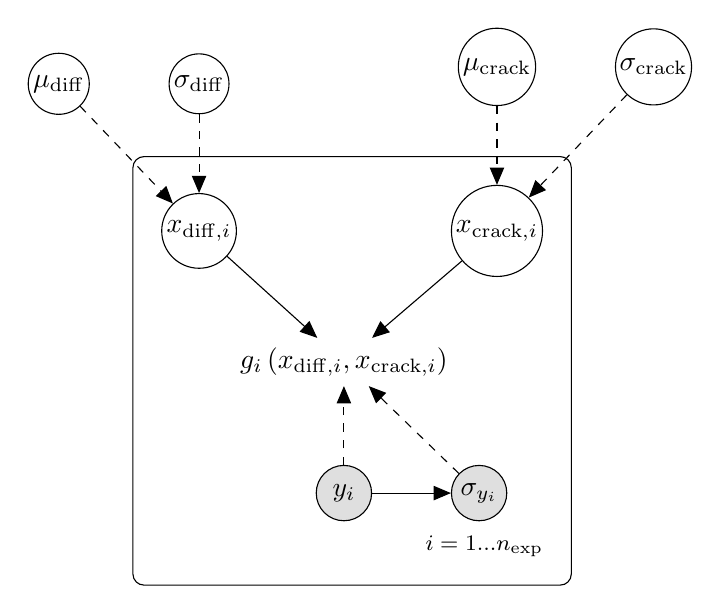
\begin{tikzpicture}
        % Input variables
        \node[latent] (x1) {$x_{\mathrm{diff}, i}$};
        \node[latent, right = of x1, draw=none] (middle) {};
        \node[latent, right = of middle] (x2) {$x_{\mathrm{crack}, i}$};
    
        % Model
        \node[rectangle, below = of middle] (M) {$g_i\left(x_{\mathrm{diff}, i},x_{\mathrm{crack}, i}\right)$};
        \edge [] {x1,x2} {M};

        % Observations
        \node[obs, below = of M] (y) {$y_i$};
        \node[obs, right = of y] (sigy) {$\sigma_{y_i}$};
        \edge [] {y} {sigy};
        \edge [dashed] {y} {M};
        \edge [dashed] {sigy} {M};

        % Represent the multiple experiments
        \plate [inner sep=1em] {N} {(x1) (x2) (y)} {$i=1...n_{\mathrm{exp}}$};

        Calibrated parameters
        \node[latent,above = of x1] (sig1) {$\sigma_{\mathrm{diff}}$};
        \node[latent, left = of sig1] (mu1) {$\mu_{\mathrm{diff}}$};
        \node[latent,above = of x2] (mu3) {$\mu_{\mathrm{crack}}$};
        \node[latent,right = of mu3] (sig3) {$\sigma_{\mathrm{crack}}$};
        \edge [dashed] {mu1,sig1} {x1};
        \edge [dashed] {mu3,sig3} {x2};     
    \end{tikzpicture}
\end{document}
